% -*- TeX:de -*-
\NeedsTeXFormat{LaTeX2e}
\documentclass[12pt,a4paper]{article}
\usepackage[english]{babel} % german text
\usepackage[DIV12]{typearea} % size of printable area
\usepackage[T1]{fontenc} % font encoding
%\usepackage[latin1]{inputenc} % most likely on Windows
\usepackage[utf8]{inputenc} % probably on Linux
\usepackage{multicol}
% PLOTTING
\usepackage{pgfplots}
\usepackage{pgfplotstable}
\usepackage{url}
\usepackage{graphicx} % to include images
\usepackage{tikz}
\usepackage{subfigure} % for creating subfigures
\usepackage{amsmath} % a bunch of symbols
\usepackage{amssymb} % even more symbols
\usepackage{booktabs} % pretty tables
\usepackage{makecell} % multi row table heading
% a floating environment for circuits
\usepackage{float}
\usepackage{caption}
\usepackage{hyperref}

% Title Page command
\newcommand{\HRule}{\rule{\linewidth}{0.5mm}}

%\newfloat{circuit}{tbph}{circuits}
%\floatname{circuit}{Schaltplan}
% a floating environment for diagrams
%\newfloat{diagram}{tbph}{diagrams}
%\floatname{diagram}{Diagramm}
\pgfplotsset{compat=1.8}
\selectlanguage{english} % use german

\begin{document}
%%%%%%% DECKBLATT %%%%%%%
\begin{titlepage}
\begin{center}

% Upper part of the page. The '~' is needed because \\
% only works if a paragraph has started.

\includegraphics[scale=0.75]{./unilogo}~\\[2cm]

\textsc{\LARGE University of Vienna }\\[0.5cm]
\textsc{\LARGE Faculty of Physics}\\[1.5cm]
\textsc{\Large Quantum optics practical course}\\[0.5cm]

% Title
\HRule \\[0.4cm]
{ \huge \bfseries Radiaton Pressure}\\[0.4cm]

\HRule \\[1.5cm]

% Author and supervisor
\begin{minipage}{0.4\textwidth}
\begin{flushleft} \large
\emph{Author:}\\
Johannes \textsc{Kurz}\\
\emph{Group:}\\
\textsc{Braun, Donabaum, Kurz}\\
\end{flushleft}
\end{minipage}
\begin{minipage}{0.4\textwidth}
\begin{flushright} \large
\emph{Supervisor:} \\
Witlef \textsc{Wieczorek}
\end{flushright}
\end{minipage}

\vfill

% Bottom of the page
{\large 31.10.2014}

\end{center}
\end{titlepage}
%%%%%%% DECKBLATT ENDE %%%%%%%
\pagebreak

\setlength{\columnsep}{20pt}
\begin{multicols}{2}

\begin{abstract}

\end{abstract}

%%%%%%%%%%%%%%%%%%%%%%%%%%%%%%%%%%%%%%%%%%%%%%%%
%\begin{figure}[H]
% \centering
% \includegraphics[scale=0.35]{./data/beugung.png}
% \caption{Beugungsmuster Einzelspalt (echtes Foto; schwarz durch weiߟ ersetzt)}
% \label{fig:beugungsmuster}
%\end{figure}

%\begin{figure}[H]
% \centering
% \pgfplotstabletypeset[
% columns={abstand, n},
% col sep=&,
% columns/abstand/.style={precision=2, zerofill, column name=\makecell{$Abstand$\\$(\pm 0.05)[mm]$} },
% columns/n/.style={column name=\makecell{$n$\\$(Ordnung)$}, precision=0},
% every head row/.style={before row=\hline,after row=\hline\hline},
% every last row/.style={after row=\hline},
% every first column/.style={column type/.add={|}{} },
% every last column/.style={column type/.add={}{|} }
% ]{
% abstand & n
% 12.9 & 1
% 24.45 & 2
% 37.40 & 3
% 49.35& 4
% 62.45 & 5
% 74.45 & 6
% 87.45 & 7
% 100.25 & 8
%
% }
% \caption{Messwerte Einzelspalt}
% \label{tab:werte_einzelspalt}
%\end{figure}
%%%%%%%%%%%%%%%%%%%%%%%%%%%%%%%%%%%%%%%%%%%%%%%%
%%%%%%%%%%%%%%%%%%%%%%%%%%%%%%%%%%%%%%%%%%%%%%%%

\section{Molecule Interference}
The aim of this experiment is to show interference patterns using $C_{60}$ molecules and the quantum mechanical description of matter waves. The following review will give you an introduction to the theory of the experiment as well as a description of the experimental setup. At the end, the obtained results are presented and discussed.

$x^2$\\

$$\sqrt{a}$$

%%%%%%%%%%%%%%%%%%%%%%%%%%%%%%%%%%%%%%%%%%%%%%%%
%%%%%%%%%%%%%%%%%%%%%%%%%%%%%%%%%%%%%%%%%%%%%%%%
\section{Theory}
\subsection{Matter Waves}
According to quantum theory, also massive particles can be described as a wave, where the wavelenght is given by the de Broglie relation.
$$\lambda=h/p$$
Thus, interference and defraction of these massive particles can be observed. The Schrödinger equation describes the propagation of such a matter wave. For time independent problems, this equation can be reduced to the Helmholtz equation. This means, that matter waves can be described as electromagnet waves and also exhibit the same effects as electromagnet waves. Thus, one can use the Talbot and the Lau effect, which are needed to perform the experiment.
\subsection{Talbot Effect}
The Talbot effect is observed in the optic near feld, or Fresnel regime, where the curvature of the wavefront can not be neglected. It occurs when coherent light impingin on a periodic grating. Then,  self images of the grating can be seen at multiples of a charactersitic distance from the grating, usually referred to as Talbot lenght. The Talbot lenght is wavelength dependend and can be calculatet by $L_T=d^2/\lambda$, where d is the grating period.

\subsection{Lau Effect}
This effect is similar to the Talbot effect but the crucial difference is that one can use an incoherent (light) source. 
%%%%%%%%%%%%%%%%%%%%%%%%%%%%%%%%%%%%%%%%%%%%%%%%
%%%%%%%%%%%%%%%%%%%%%%%%%%%%%%%%%%%%%%%%%%%%%%%%
\section{Experimental assembly}
The following figure shows a sketch of the experimental setup. The setup is divided into 3 compartments. The first part contains the oven (which is the source of the molecules) as well as the chopper and delimiters which are needed for the velocity selection. 
After the source chamber, the molucule beam enters the inteferometer chamber. In this part, the 3 gratings are situated. $G_1$ and $G_3$ are silicon nitride gratings with perodicity of 266nm. $G_2$ is a standing light wave produced by a 532nm Laser (which results in a 266nm periodicity, too).
The third and last compartment contains an electron inoization quadrupol mass spectrometer where the interference patterns are detected.
In order to get the intended result, the whole experiment takes place in vacuum. This ensures that the molecules do not collide with atoms of the background gas.

The oven itself is a ceramic cylinder which is secluded by a stainless steel top cover and heated by a heating wire. It is used to evapourate the molecules. In our case, it was filled with $C_{60}$ molecules. The apparatus is mounted on a translation stage, thus, the direction of the beam can be moduled in the X/Y axis via joystick.
In order to get a temporal coherent beam, a velocity selection has to be made. 
At the beginning of the experiment, the oven is heated up until it has reached a stable temperature of about $620^\circ$. Then, the joystick was used to optimize the countrate.


%%%%%%%%%%%%%%%%%%%%%%%%%%%%%%%%%%%%%%%%%%%%%%%%
%%%%%%%%%%%%%%%%%%%%%%%%%%%%%%%%%%%%%%%%%%%%%%%%
\section{Results}




%\begin{figure}[H]
%	\centering
%	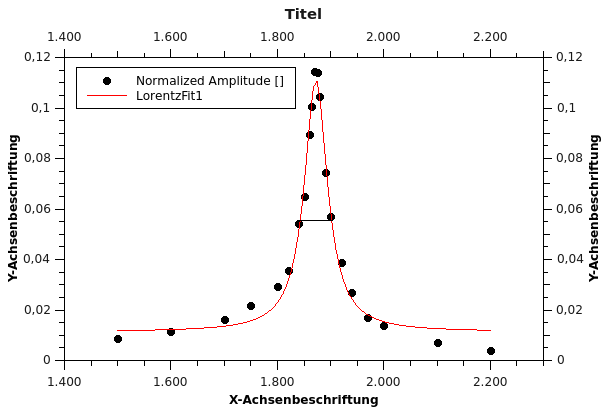
\includegraphics[scale=1]{../figures/Resonanzkurve.png}
%	\caption{Resonanzkurve}
%	\label{fig:resonanzkurve}
%\end{figure}

%%%%%%%%%%%%%%%%%%%%%%%%%%%%%%%%%%%%%%%%%%%%%%%%
%%%%%%%%%%%%%%%%%%%%%%%%%%%%%%%%%%%%%%%%%%%%%%%%
\section{Discussion}


\section{Resources}
\begin{itemize}
	\item SImulation of the Experiment \url{http://www.univie.ac.at}
\end{itemize}
%\bibliography{protocol.bib}
%\bibliographystyle{plain}

\end{multicols}
\end{document}